\section{Dense attention trains unreliably on this recipe}
\label{sec:dense}

The dense baseline was the least reliable model in the study. On the isolated data, dense attention transitioned
within 60 epochs on two of the four seeds we tried (two of seven runs, counting reruns in float32); the $S_1{=}6$ selector
transitioned on all four seeds, and the selector as a whole in 11 of 12 M5-profile runs (Figure~\ref{fig:dense}). When dense did transition it reached 1.000, so this is a finding about training
reliability within a fixed budget, not about recall capacity.

\begin{figure}[t]
\centering
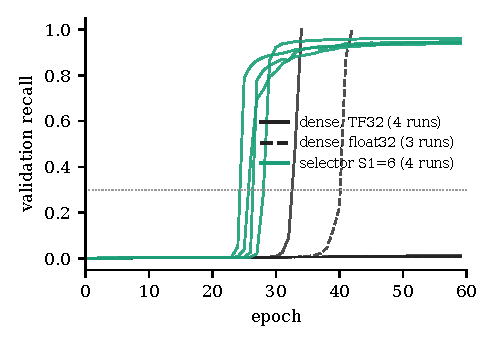
\includegraphics[width=0.6\linewidth]{figures/fig2_training.pdf}
\caption{\textbf{On identical data, the sparse selector learned every time and dense attention mostly did not.}
Validation recall per epoch for the seven dense runs (solid: TF32; dashed: float32) and four $S_1{=}6$ runs on
seeds 123 and 810001--810003, isolated data. The dotted line is the 0.30 transition threshold. One float32 dense run
(seed 810001) was stopped after 55 of 60 epochs.}
\label{fig:dense}
\end{figure}

\paragraph{Neither numerics nor the data generator alone explains it.} M5 changed two things at once relative to
M4: TF32 matrix multiplication and the isolated data generator. On seed 123 we separated them
(Table~\ref{tab:densecheck}). Dense learned under TF32 with the legacy data (transition at epoch 26, 0.987) and in
float32 with the isolated data (epoch 41, 1.000). With one run per cell, this is consistent with the isolated data delaying
the transition, and with ordinary seed-level chance; the pre-registered reading allowed both. We then reran dense in float32 on the two reserved seeds where it had failed. Neither
transitioned: seed 810003 finished at 0.0069 held-out recall, and seed 810001 was stopped at epoch 55 of 60 with best
validation recall 0.0068, so it has no held-out score.

\begin{table}[t]
\centering
\small
\begin{tabular}{llrr}
\toprule
Numerics & Data generator & held-out recall & transition epoch \\
\midrule
float32 & legacy (M4) & 0.992 & 28 \\
TF32 & legacy & 0.987 & 26 \\
float32 & isolated & 1.000 & 41 \\
TF32 & isolated (M5) & 0.010 & never \\
\bottomrule
\end{tabular}
\caption{\textbf{Dense learned under each change alone, but late on the isolated data.} Dense attention, seed 123,
one run per row. Row 1 is the M4 follow-up (earlier code revision); rows 2 and 3 were run to separate the two
changes made between M4 and M5.}
\label{tab:densecheck}
\end{table}

\paragraph{What this means for the comparison.} One explanation is that dense attention's phase transition on this
task arrives at a time that varies widely with the data draw and the numerics, and that our 60-epoch budget cuts off
the late cases. Two observations caution against reading this as only a matter of time. The cosine schedule brings
the learning rate close to zero by epoch 60, so a longer ceiling would also change the schedule. And in every failed
dense run validation loss reached its minimum between epochs 16 and 21 and then rose; in the float32 reruns training
loss kept falling, to about 7.2 against about 8.1 on validation, a pattern consistent with memorising the 20{,}000
training sequences. We did not test either explanation, and we did not change the recipe after seeing the data. The comparison is also not perfectly matched: the dense baseline applies dropout 0.1 inside
attention and the selector does not, and the two mixers differ in parameters (the selector adds branch gates).
Either difference could affect when the transition arrives. Its consequence is concrete: on seeds 810001 and 810003 the selector learned (0.937 and 0.945 at
$S_1{=}6$) where full attention, on identical data and recipe, did not. It also means the study has a single valid
dense-versus-selector pair (seed 810002), which is why we report its gaps as observations rather than estimates.
